%************************************************
\chapter{Appendix}\label{ch:appendix}

\section{Separating Axis Theorem}

This method determines if two convex shapes intersect. It can be also used to calculate the minimum penetration vector but we are only interested in knowing if two shapes overlap. Even though we will be working with two-dimensional shapes, it is also applicable to 3 dimensional objects. \cite{ericson2004real}

The idea behind the algorithm is that if two shapes are not intersecting, then there is an axis that separate both without touching them. It tests a number of axes, looking for the one that meets the condition. 

To determine if an axis does separate the shapes, both of them are projected onto the perpendicular line to the axis. By doing this, we reduce in one dimension the problem and now it is only necessary to check if the projections intersect. In one dimension, they overlap if at least one of the extremes of one of them is between the extremes of the other projection.

The number of axes that could be separating axis is high, but the algorithm will not check them all. For this matter, every axis is equivalent to one of the axes parallel to the edges of the shapes. In our specific case, since all the shapes the game uses are regular rectangles and the rotation is also known before hand, we can skip this step. Instead of calculating the parallel axis to all edges, we project shapes in four axes: one corresponding with $x$ axis, another with $y$ axis, 25º or -25º. Every allowed rotation will use one of these four. 

To project the blocks into the axes, we perform a dot product operation between the axis and the vertices. The maximum and minimum will be the extremes of the projection. 

\section{Visualization of results in games}

% NEED FORMATTING
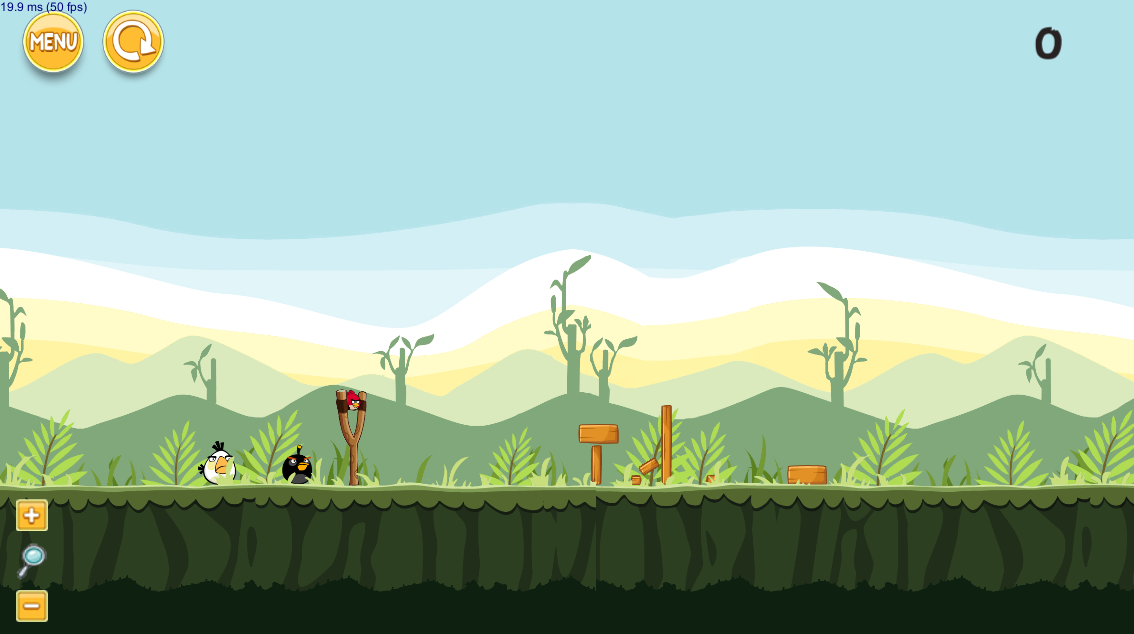
\includegraphics[scale=0.3]{gfx/e1/level-0-180522_171359.png}
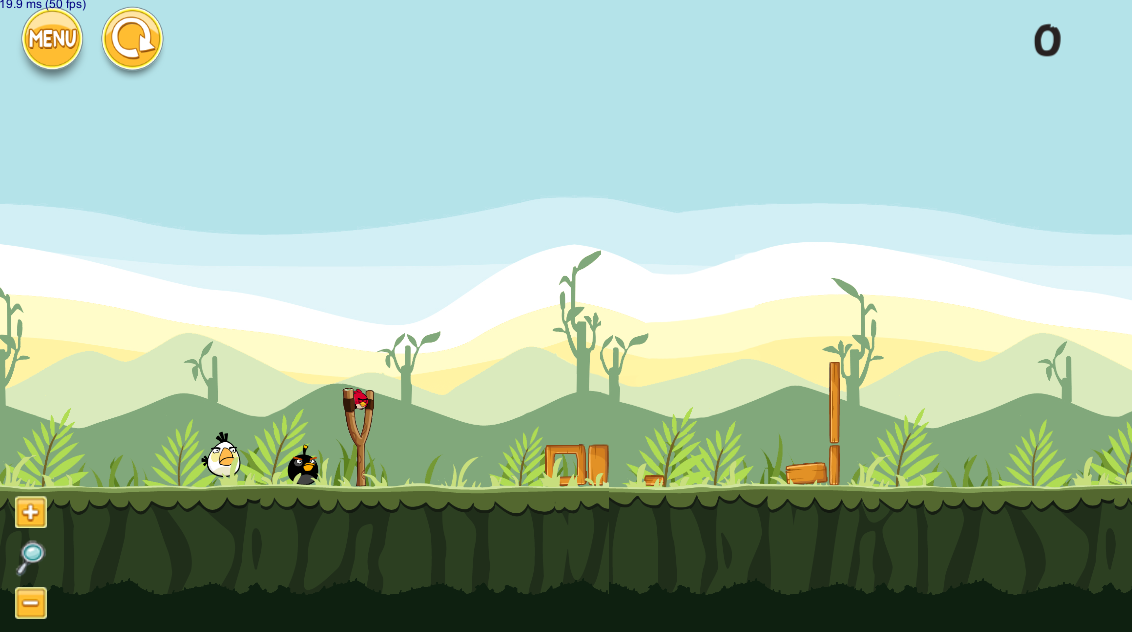
\includegraphics[scale=0.3]{gfx/e1/level-0-180522_183913.png}
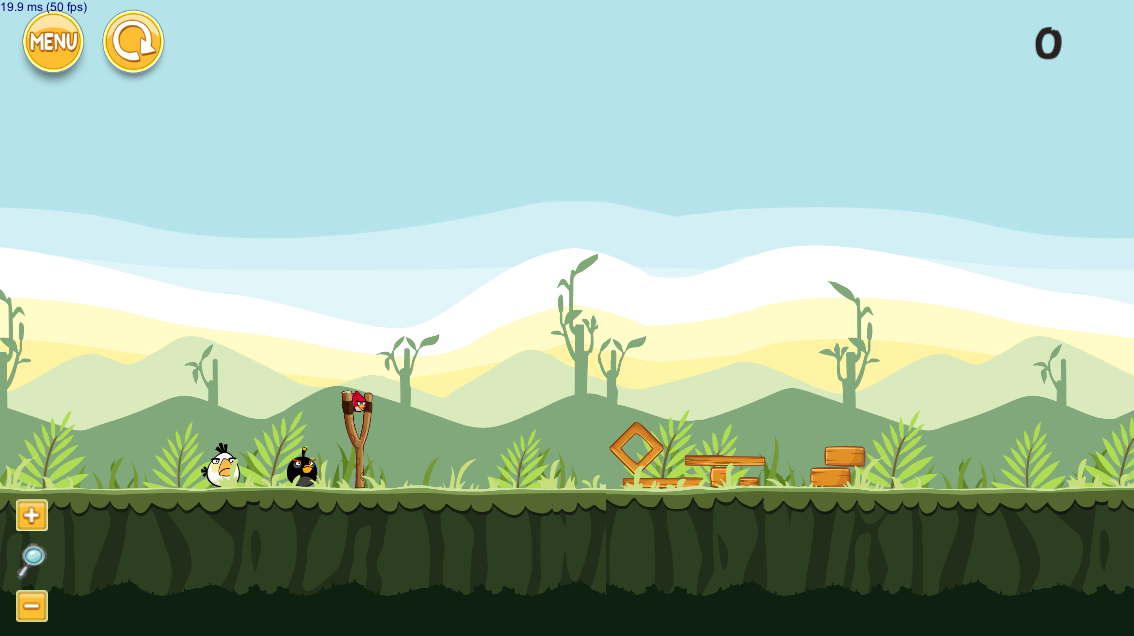
\includegraphics[scale=0.3]{gfx/e1/level-0-180523_194214.png}
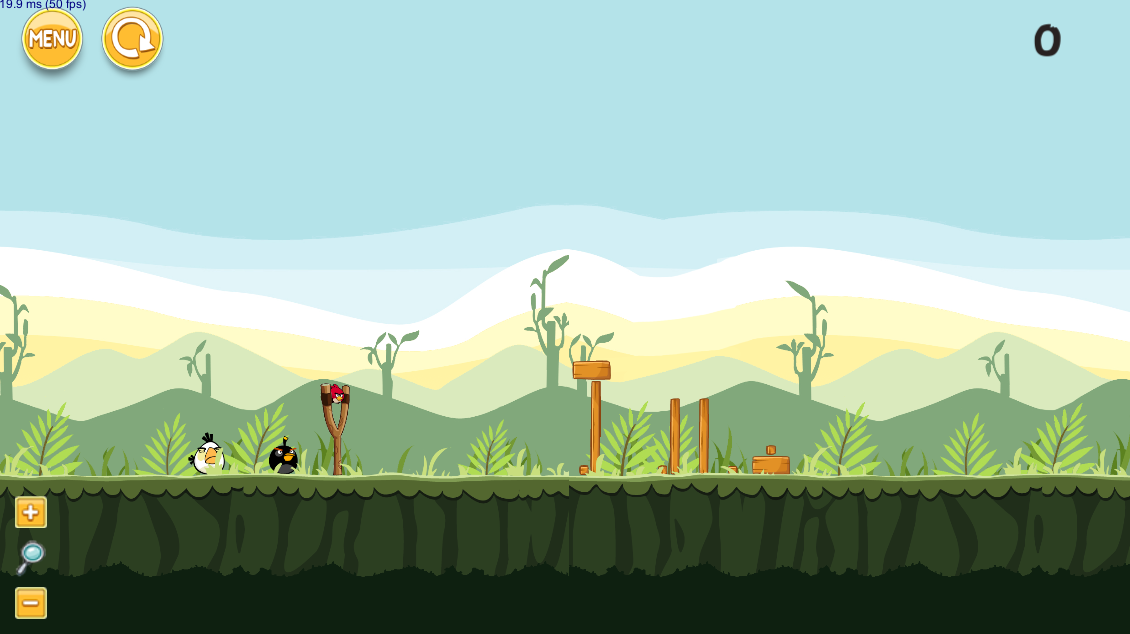
\includegraphics[scale=0.3]{gfx/e1/level-0-180523_203106.png}
%************************************************

%*****************************************
%*****************************************
%*****************************************
%*****************************************
%*****************************************
